\section{Flexible Resource Allocation Mechanisms}
\label{sec:flexible-resource-allocation-mechanisms}
As explained in the last Section, all previous research outlined in Section~\ref{sec:related-work} is incompatible
with our resource elastic optimisation problem in Section~\ref{sec:problem-formulation}. Therefore in this
section, we propose three mechanisms for solving this optimisation problem: an approximation algorithm and two
auction-based mechanisms. \\
The optimisation problem is a extended version of the knapsack problem, which is often solved using an dynamic
programming method that has pseudo-polynomial time complexity~\cite{toth1980dynamic}. The solution requires building
a table of items to bags allocation. For our problem, as the resource speeds must be considered at the same time, this
makes such a solver infeasible due to both the space and time complexity required.

Because of this issue of allocating both tasks to a server and a server's resources to a task, this work proposes an
approximation algorithm where tasks are allocated to a server with resources in series not in parallel. The centralised
greedy algorithm (detailed in Subsection~\ref{subsec:greedy-algorithm}) ranks tasks that are each allocated to a server
with resources that at each stage uses a separate ranking function. This algorithm has a social welfare lower bound
of $\frac{1}{\left|J\right|}$, however in practice achieves close to the theoretical optimal while running with
polynomial time complexity.

As task users can be self-interested, they may report their task values or requirements strategically. Traditionally,
VCG~\cite{vickrey,Clarke,groves} is used for such systems due to its ability to use any optimisation problem to
calculate a task price. However, due to the difficulty of calculating the optimal allocation for this problem, VCG is
infeasible to use in this application. Therefore, to deal with self-interested users, we propose two auction-based
mechanisms. The first being an incentive-compatible auction using the centralised greedy algorithm
(Section~\ref{subsec:critical-value-auction}) and the second being a novel Decentralized Iterative
Auction (Section~\ref{subsec:decentralised-iterative-auction}) that does not require users to reveal the task value.

\subsection{Greedy Algorithm}
\label{subsec:greedy-algorithm}
To solve a knapsack problem, a greedy approximation algorithm is often used~\cite{sahni1975approximate}. We have
applied a similar approach to this problem specified in subsection~\ref{subsec:optimisation-problem}. As a result of
the elastic nature of task resources, an additional stage is required once a task has been allocated to a server in
order to determine the task's resource speeds.

\begin{wrapfigure}{r}{0.5\linewidth}
    \centering
    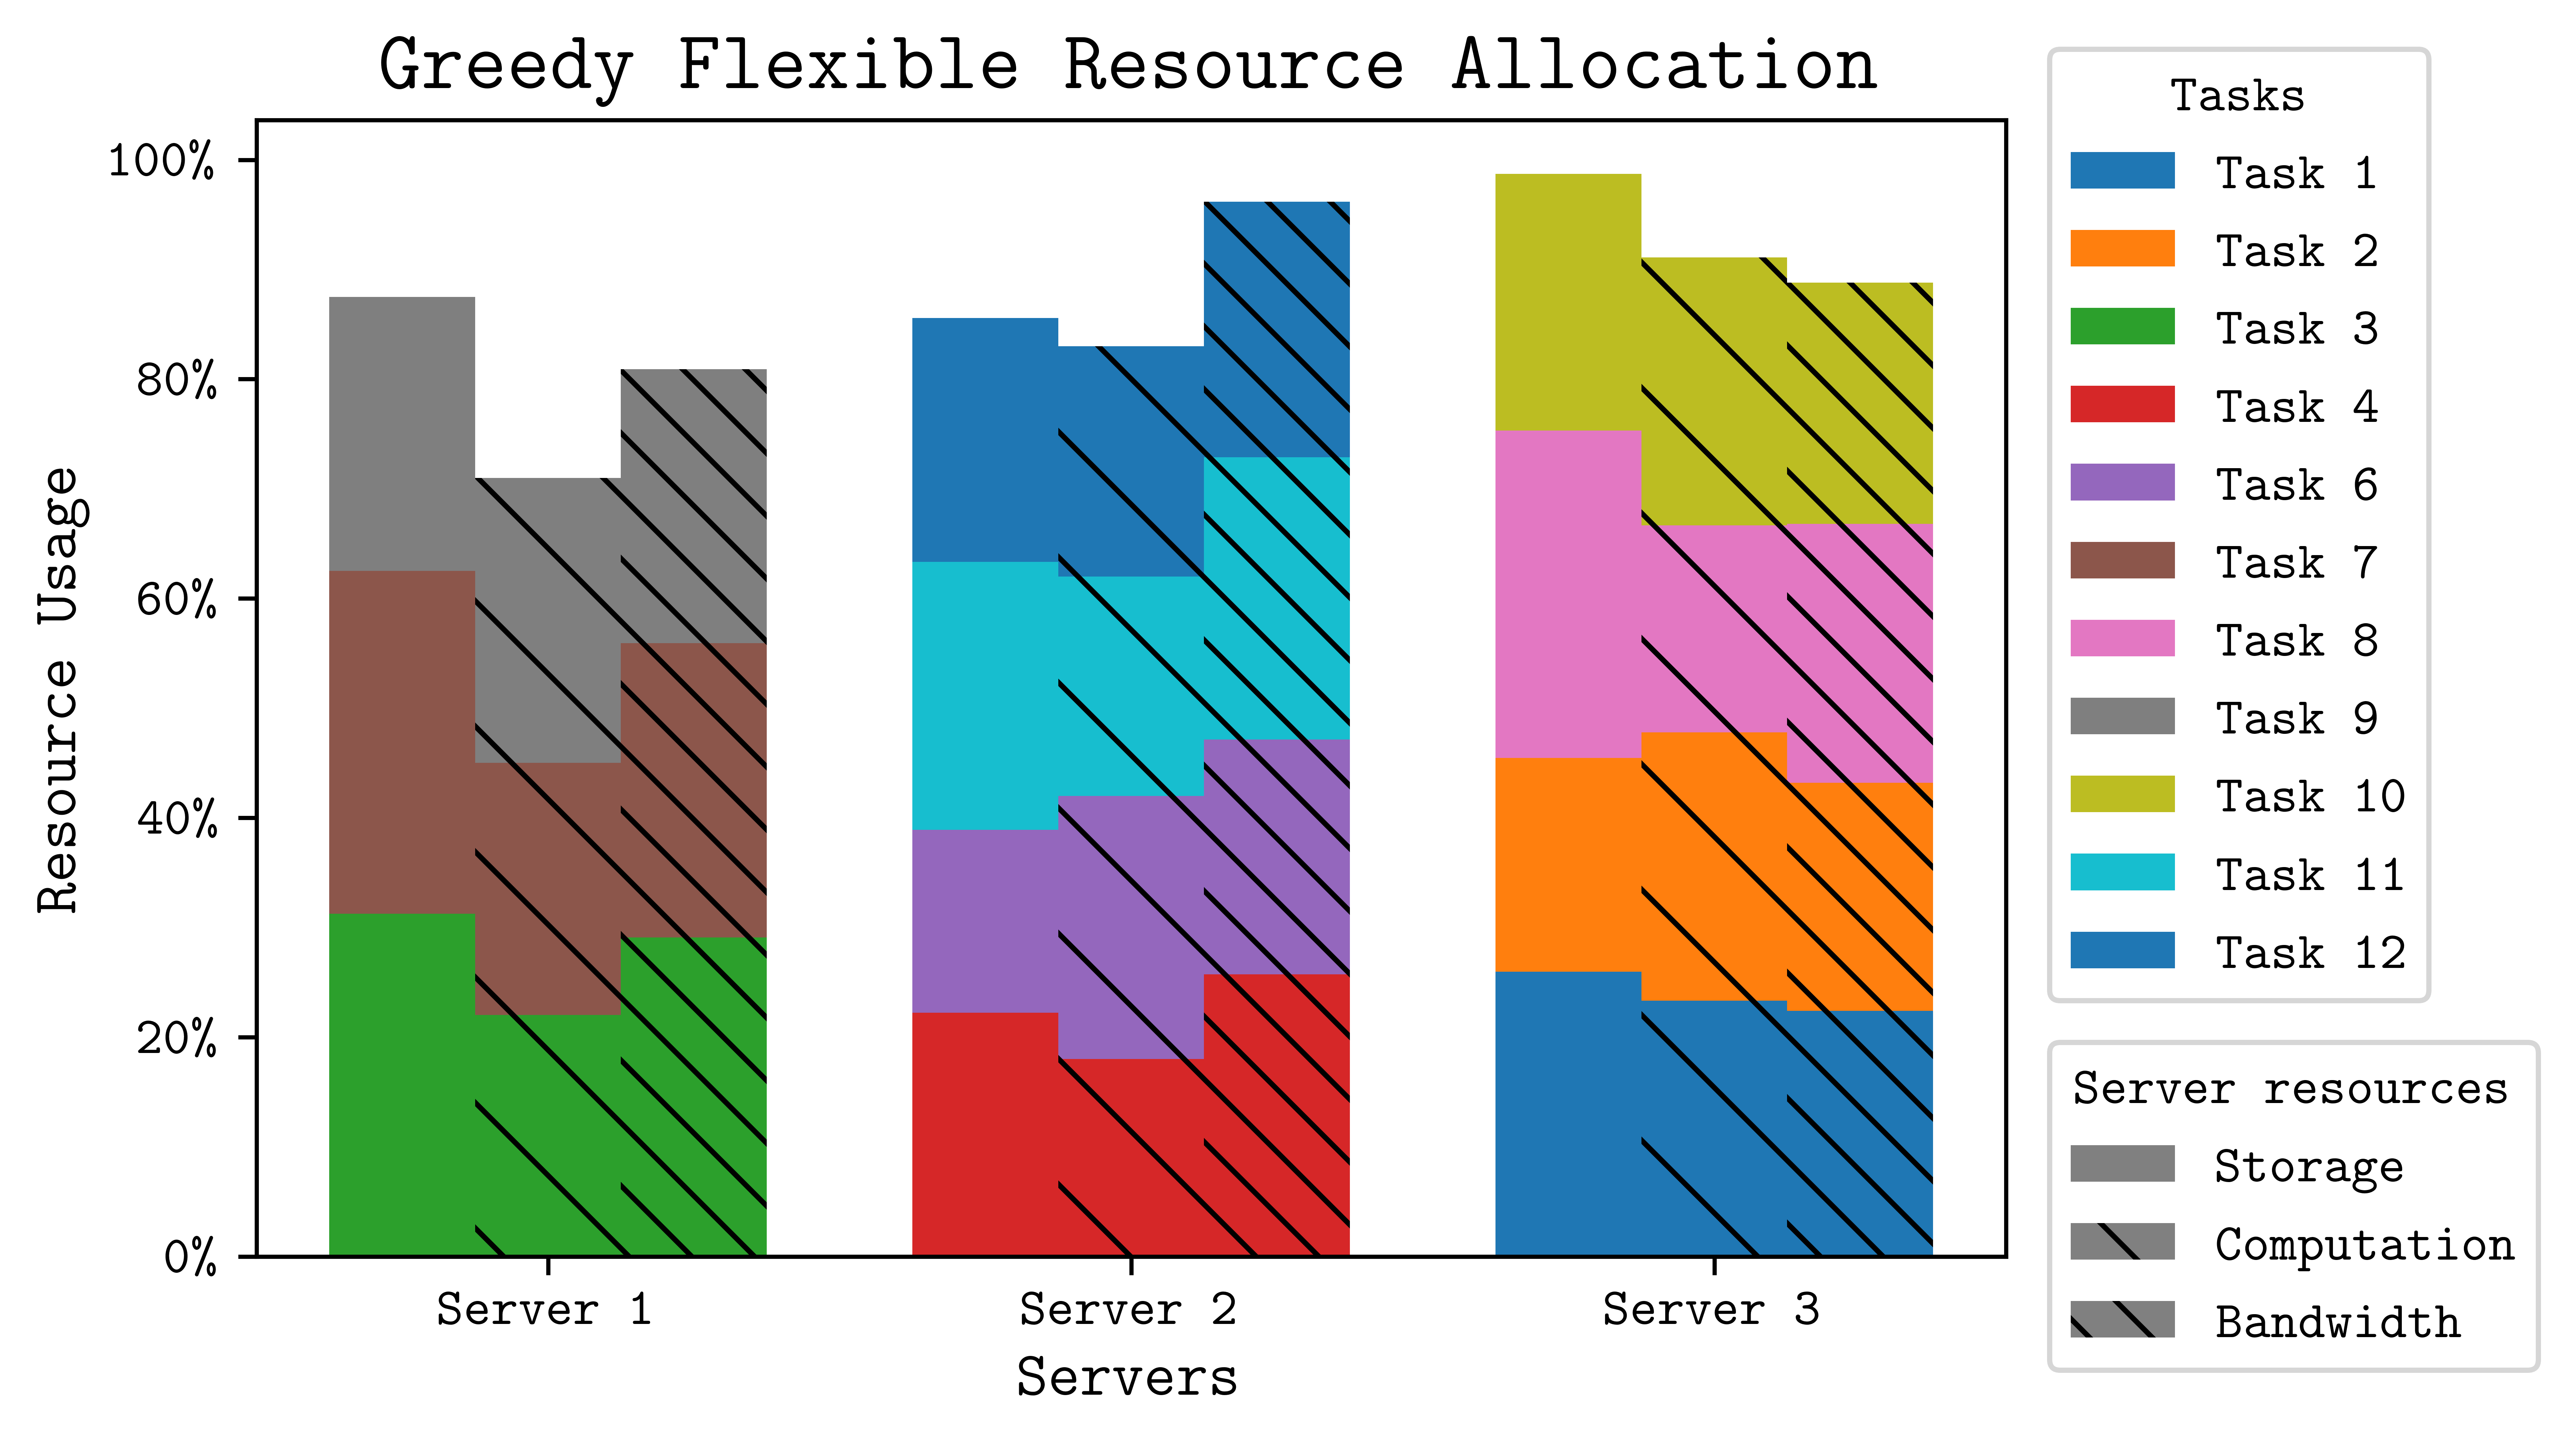
\includegraphics[width=\linewidth]{figs/allocation/greedy_flexible_resource_allocation.png}
    \caption{Example Greedy allocation using the model from table~\ref{tab:example-tasks-server-properties}
             with task and server attributes}
    \label{fig:example-greedy-allocation}
\end{wrapfigure}

More specifically, the greedy algorithm (algorithm~\ref{alg:greedy-algorithm}) has two stages; stage one sorts the list
of tasks based on the value density of each task calculated using task attributes: value, required resources and
deadline. The second stage uses the sorted list of tasks to iterate through applying two heuristics to select the
server based on available server resources and to allocate resources based on the available server resources and the
required resources of the task.

Using the same example case from subsection~\ref{subsec:example-problem-case}, the greedy algorithm can complete 12/12 of
the tasks achieving 21\% more social welfare than the fixed solution, same as the optimal flexible solution.
The greedy algorithm uses the value density function:
\[\frac{v_j \cdot d_j}{s_j + w_j + r_j}\] server selection:
 \[\text{argmin}_{\forall i \in I} S^{'}_i \cdot W^{'}_i \cdot R^{'}_i\] for task $j$ and servers $I$ and the resource allocation:
\[\text{argmin}_{s^{'}_j, w^{'}_j, r^{'}_j} \left(\frac{w^{'}_j}{W^{'}_i}\right)^3 + \left(\frac{s^{'}_j + r^{'}_j}{R^{'}_i}\right)^3\]
is task $j$ and server $i$.

\begin{algorithm}
    \caption{Pseudo code of Greedy Algorithm}
    \label{alg:greedy-algorithm}
    \begin{algorithmic}
        \REQUIRE $J$ is the set of tasks and $I$ is the set of servers
        \REQUIRE $S^{'}_i$, $W^{'}_i$ and $R^{'}_i$ is the available resources
            (storage, computation and bandwidth respectively) of server $i$
        \REQUIRE $v(j)$ is the value density function of task $j$
        \REQUIRE $s(j, I)$ is the server selection function of task $j$ and set of servers $I$ returning the best
            server, or $\emptyset$ if the task is not able to be run on any server
        \REQUIRE $r(j, i)$ is the resource allocation function of a task and server returning a tuple of the
            loading, compute and sending speeds
        \REQUIRE $\text{sort}(X, f)$ is a function that returns a sorted list of elements in descending order, based
            on a set of elements $X$ and a function for comparing elements $f$

        \STATE{$J^{'} \leftarrow sort(J, v)$}
        \FORALL{$j \in J^{'}$}
            \STATE{$i \leftarrow s(j, I)$}
            \IF{$i \neq \emptyset$}
                \STATE{$s^{'}_j, w^{'}_j, r^{'}_j \leftarrow \gamma(j, i)$}
                \STATE{$x_{i,j} \leftarrow 1$}
            \ENDIF
        \ENDFOR
    \end{algorithmic}
\end{algorithm}

\subsubsection{Greedy Lower Bound}
\label{subsubsec:greedy-lower-bound}
The lower bound of the algorithm is $\frac{1}{\left|J\right|}$ (where $\left|J\right|$ is the number of tasks) with
the task value as the value density function. This lower bound is not affected by the server selection policy or the
resource allocation policy. \\
However in testing, we found that the task value function is not the best value density heuristic as it does not
consider the effect of deadlines or the required resources of the task. In Section~\ref{sec:empirical-results}, we
considered a wide range of heuristics, showing the results of the best heuristics over a range of settings.

\begin{theorem}
    The lower bound of the greedy algorithm is $\frac{1}{n}$ of the optimal social welfare.
\end{theorem}
\begin{proof}
    Due to a task not considering other task's resource requirements when allocating resources then no matter the
    server selection or resource allocation function, it can not be guaranteed that any subsequent tasks could be
    allocated to any server after the first task is allocated.
    As a result, the algorithm can be guaranteed to achieve at least $\frac{1}{n}$ of the optimal social
    welfare by sorting the tasks by task value ($v(j) = j_v$). Using this, the first task from the sorted task list
    will have the maximum task value meaning the lower bound of the algorithm is $\frac{1}{n}$ of the optimal social
    welfare.
\end{proof}

\subsubsection{Greedy Time Complexity}
\label{subsubsec:greedy-time-complexity}
Using the greedy algorithm (algorithm~\ref{alg:greedy-algorithm}), the time complexity is polynomial,
$O(\left|J\right| \left|I\right|)$.
\begin{theorem}
    Time complexity of the greedy algorithm is $O(\left|J\right| \left|I\right|)$, where $\left|J\right|$ is the number
    of tasks and $\left|I\right|$ is the number of servers. Assuming that the value density and resource allocation
    heuristics have constant time complexity and the server selection function is $O(\left|I\right|)$.
\end{theorem}
\begin{proof}
    The time complexity of stage 1 of the algorithm is $O(\left|J\right| \log(\left|J\right|))$ due to sorting the
    tasks and stage 2 has complexity $O(\left|J\right| \left|I\right|)$ due to looping over all the tasks and
    applying the server selection and resource allocation heuristics. Therefore the overall time complexity is
    $O(\left|J\right| \left|I\right| + \left|J\right| \log(\left|J\right|) = O(\left|J\right| \left|I\right|)$.
\end{proof}

\subsection{Critical Value Auction}
\label{subsec:critical-value-auction}
Due to the problem case being non-cooperative, if the greedy algorithm was used to allocate resources such that the
value is the price paid, this would be open to manipulation and misreporting of task attributes like the value,
deadline or resource requirements. Therefore, in this section we propose an auction that is strategy-proof
(weakly dominant incentive compatible) so users have no incentive to misreport task attributes.

Single-Parameter domain auctions are extensively studied in mechanism design~\cite{nisan2007algorithmic_228} and are
used where an agent's valuation function can be represented as a single value. The task price is calculated by finding
the critical value, the minimum task price required for the task still allocated to any server. This has
been shown to be a strategy-proof~\cite{nisan2007algorithmic_229_230} auction making it a weakly dominant strategy for
all users to honestly reveal their task attributes.

\begin{algorithm}
    \caption{Pseudo code of the Critical Value Auction}
    \label{alg:critical-value-auction}
    \begin{algorithmic}
        \REQUIRE $J$ is the set of tasks and $I$ is the set of servers
        \REQUIRE $S^{'}_i$, $W^{'}_i$ and $R^{'}_i$ is the available resources
            (storage, computation and bandwidth respectively) of server $i$
        \REQUIRE $v(j)$ is the value density function of task $j$
        \REQUIRE $v^{-1}$ is the inverse of the value density function making the value the subject of the function
        \REQUIRE $s(j, I)$ is the server selection function of task $j$ and set of servers $I$ returning the best
            server, or $\emptyset$ if the task is not able to be run on any server
        \REQUIRE $r(j, i)$ is the resource allocation function of a task and server returning a tuple of the
            loading, compute and sending speeds
        \REQUIRE $\text{sort}(X, f)$ is a function that returns a sorted list of elements in descending order, based
            on a set of elements $X$ and a function for comparing elements $f$
        \REQUIRE $\text{can\_allocate}(j, I)$ determines whether task $j$ can be allocated to any server $I$
        \REQUIRE $\text{Greedy}(J, I, v, s, r)$ is the greedy algorithm (subsection~\ref{subsec:greedy-algorithm}) with
            tasks $J$, servers $I$, value density $v$, server selection policy $s$, resource allocation policy $r$.

        \STATE{$\text{Greedy}(J, I, v, s, r)$}
        \FORALL{$j^{'} \in \{j \in J | \exists x_{j, i} \forall i \in I\}$}
            \FORALL{$j \in J$}
                \IF{$j^{'} \neq j$}
                    \STATE{$i \leftarrow s(j, I)$}
                    \IF{$i \neq \emptyset$}
                        \STATE{$s^{'}_j, w^{'}_j, r^{'}_j \leftarrow \gamma(j, i)$}
                    \ENDIF
                    \IF{$\neg \text{can\_allocate} (j^{'}, I)$}
                        \STATE{$p_{j^{'}} \leftarrow v^{-1}(v(j), j^{'})$}
                    \ENDIF
                \ENDIF
            \ENDFOR
        \ENDFOR
    \end{algorithmic}
\end{algorithm}

The auction (specified in algorithm~\ref{alg:critical-value-auction}) is implemented using the greedy algorithm from
subsection~\ref{subsec:greedy-algorithm} both in finding the initial allocation and critical value for each task (at
least in a modified form). This is helpful as it allows the auction to inherit many of the properties of the greedy
algorithm like social welfare and time complexity.
By running the greedy algorithm with all of the tasks' reported values then an initial allocation can be found. Then for
each task that was allocated the critical value for the task must be found meaning that the task will pay the minimum
possible value (price) such that the task would still have been allocated by the greedy mechanism. \\
To find the critical value of the task (referred to here as the critical task) is relatively simple by just modifying
the greedy algorithm. So when looping through the list of tasks sorted by value density, the critical task is ignored
here, once a task is allocated to a server with resources a check is done to see if the critical task could be
allocated to any server. This check has linear time complexity as it is assumed that the server could allocate all of
its available resources to the task, only requiring the bandwidth resources to split between loading and sending speeds.
Therefore a linear search is required to check if any split would allow the task to be completed. \\
This process of allocating tasks and checking if the critical task could be allocated is repeated till the critical
task can't be allocated to any server. At which point, the value density of the task just allocated is equal to the
minimum value density of the critical task such that the critical task could have been allocated. Using this
information, the critical value is equal to the inverse of the value density function (where the value is the subject
of the function not the value density) using the value density of the previously allocated task's value density.

\subsubsection{Critical Value Auction Time Complexity}
\label{subsubsec:critical-value-auction-time-complexity}
The time complexity of the auction is $O(\left|J\right| \left|J\right| \left|I\right|)$, the greedy
algorithm repeated $\left|J\right|$ due to calculating each task's critical value.
\begin{theorem}
    The time complexity of the critical value auction is $O(\left|J\right| \left|J\right| \left|I\right|)$.
\end{theorem}
\begin{proof}
    As explained more fully in subsection~\ref{subsec:critical-value-auction}, the auction uses the greedy algorithm
    (subsection~\ref{subsec:greedy-algorithm}) that has time complexity $O(\left|J\right| \left|I\right|)$. The
    auction then repeats a modified version of the greedy algorithm for each task allocated initially such that after
    each task is allocated a check is done to see if the current task could be allocated to any server. This is done by
    repeating the server selection and resource allocation functions for each task (excluding the critical task) with
    time complexity, $O(\left|J\right| \left|I\right|)$, until the critical task can no longer be allocated to any
    server (a linear time function). The task's critical value is calculated in constant time function. As a result,
    the time complexity for calculating the critical value for an individual task is $O(\left|J\right| \left|I\right|)$.
    Thus, the overall time complexity is $O(\left|J\right| \left|J\right| \left|I\right|)$ due to the critical value
    being found for every task.
\end{proof}

\subsubsection{Demonstrating that the Critical Value Auction is Strategyproof}
\label{subsubsec:critical-value-auction-strategyproof}
In order to make the auction strategyproof, the value density function must be
monotonic~\cite{nisan2007algorithmic_229_230}. This ensures that if a task misreports any attributes, it will result
in the value density of the task decreasing, increasing the price paid. Therefore a value density function must be in
the form of $\frac{v_j \cdot d_j}{\alpha(s_j, w_j, r_j)}$ such it is monotonic decreasing if a task attribute is
misreported.
\begin{theorem}
    The value density function $\frac{v_j \cdot d_j}{\alpha(s_j, w_j, r_j)}$ is monotonic increasing for task $j$
    assuming the function $\alpha(s_j, w_j, r_j)$ is monotonic increasing for each variable.
\end{theorem}
\begin{proof}
    In order to misreport the task value and deadline, misreported values must be less than their true value. Therefore
    if the value or deadline are decreased then the value density will likewise decrease. \\
    The opposite is true for a task's required resources (storage, compute and result data), as the misreported value
    must be greater than the true value otherwise the task would not be able to be completed. Therefore as the $\alpha$
    function will increase as the resource requirements increase, the resulting value density will decrease. \\
    So in all cases, the overall value density will decrease if the owner does not accurately report a task's attribute,
    making the function monotonic.
\end{proof}

\subsection{Decentralised Iterative Auction}
\label{subsec:decentralised-iterative-auction}
In some applications of edge cloud computing, keeping the value of a task a secret is important, for example in
military-tactical networks. Therefore we propose a novel Decentralised Iterative Auction based on the pricing principle
of the VCG auction~\cite{vickrey,Clarke,groves}. VCG auction calculates the price of an item by finding the
difference in social welfare if the item exists and when it does not exist.

Our proposed novel auction uses the same principle, except in reverse by finding the difference between the current
server revenue and the revenue when the task is allocated with a price of zero. To cause the overall revenue and
server revenue to increase, a small value called the Price change variable is added to the task price.

Our auction uses this principle by iteratively letting a task advertise its requirements to all the servers, who
respond with their price to run the task. This price is equal to the server's current revenue minus the solution to the
problem in subsection~\ref{subsubsec:decentralised-iterative-problem} plus the price change variable. This is done to
ensure that the total server revenue increases by accepting the task. Once all of the servers have responded, the task
can compare the minimum server prices to its private evaluation. This allows the task to privately select the server
that it runs on (assumed to be the server with the lowest price) otherwise the task will stop advertising as it knows
that its evaluation is lower than the price of any server.

An additional heuristic is used as well to reduce the number of rounds required to find the revenue optima at setting
an initial price for a task. This is useful to account for the minimum costs of running the task. The heuristic
is referred to as the Initial Price which is set individually by each server.

The algorithm~\ref{alg:dia} is a centralised version of the auction. The auction runs iteratively till no task is left
so either the task can't be allocated to any server or is allocated to a server for a price. In this centralised version,
a random task is selected which is then advertised to all of the server who each solve the problem in
subsection~\ref{subsubsec:decentralised-iterative-problem} to calculate the task price. The minimum price returned by
$P(i, k)$ is compared to the task's reverse price (the maximum amount the task is willing to pay). If the price is less
than the task value then the task is allocated to the minimum price server and the task price set to the agreed price.
Otherwise the task is removed from the set of tasks to be allocated. In the process of allocating a task to a server
could result in some other tasks being deallocated from the server. These deallocated tasks are then added back to the
set of tasks to be allocated to be selected again.

\begin{algorithm}
    \caption{Decentralised Iterative Auction}
    \label{alg:dia}
    \begin{algorithmic}
        \REQUIRE $I$ is the set of servers
        \REQUIRE $J$ is the set of unallocated tasks, that is initial the set of all tasks
        \REQUIRE $P(i, k)$ is the solution to the problem in section~\ref{subsubsec:decentralised-iterative-problem}
            using the server $i$ and new task $k$. The server's current tasks is known to itself and its current
            revenue from tasks so not passed as arguments.
        \REQUIRE $\leftarrow_R$ will randomly select an element from a set

        \WHILE{$|J| > 0$}
            \STATE{$j \leftarrow_R J$}
            \STATE{$p, i \leftarrow \min_{i \in I} P(i, j)$}
            \IF{$p \leq v_j$}
                \STATE{$p_j \leftarrow p$}
                \STATE{Allocate task $j$ to server $i$}
                \STATE{Add tasks deallocated from server $i$ back to $J$}
            \ENDIF
            \STATE{$J \leftarrow J \setminus \{j\}$}
        \ENDWHILE
    \end{algorithmic}
\end{algorithm}

\subsubsection{Server revenue optimisation problem}
\label{subsubsec:decentralised-iterative-problem}
To find the optimal revenue for a server $m$ given a new task $n^{'}$ and a set of currently allocated tasks $N$ has a
similar formulation to the optimisation problem in section~\ref{subsec:optimisation-problem}. Except with an additional
variable for the task price $p_n$ for each task $n$.

\begin{align}
    \max & \sum_{\forall n \in N} p_n x_n\label{eq:dia-objective}\\
    \mbox{s.t.} \nonumber \\
    & \sum_{\forall n \in N} s_n x_n + s_{n^{'}} \leq S_m,\label{eq:dia-server-storage-constraint}\\
    & \sum_{\forall n \in N} w^{'}_n x_n + w_{n^{'}} \leq W_m, \label{eq:dia-server-computation-constraint}\\
    & \sum_{\forall n \in N} (r^{'}_n + s^{'}_n) \cdot x_n + (r^{'}_{n^{'}} + s^{'}_{n^{'}}) \leq R_m, \label{eq:dia-server-communication-constraint}\\
    & \frac{s_n}{s^{'}_n} + \frac{w_n}{w^{'}_n} + \frac{r_n}{r^{'}_n} \leq d_n, &~ \forall n \in N \cup \{n^{'}\} \label{eq:dia-task-deadline}\\
    & 0 < s^{'}_n < \infty, &~ \forall{n \in N \cup \{n^{'}\}} \label{eq:dia-loading-speeds}\\
    & 0 < w^{'}_n < \infty, &~ \forall{n \in N \cup \{n^{'}\}} \label{eq:dia-compute-speeds}\\
    & 0 < r^{'}_n < \infty, &~ \forall{n \in N \cup \{n^{'}\}} \label{eq:dia-sending-speeds}\\
    & x_n \in \{0,1\} &~ \forall{n \in N} \label{eq:dia-task-allocation}
\end{align}

The objective (Eq.~\eqref{eq:dia-objective}) is to maximize the price of all currently allocated tasks (not including
the new task as the price is zero). The server resource capacity constraints
(Eqs.~\eqref{eq:dia-server-storage-constraint},~\eqref{eq:dia-server-computation-constraint}
and~\eqref{eq:dia-server-communication-constraint}) are similar to the constraints in the standard model set out in
section~\ref{subsec:optimisation-problem} except with the assumption that the task $n^{'}$ is running. The deadline and
non-negative resource speeds constraints (\ref{eq:dia-task-deadline},~\ref{eq:dia-loading-speeds}
,~\ref{eq:dia-compute-speeds} and~\ref{eq:dia-sending-speeds}) are all the same equation as the standard formulation
for all the tasks plus the new task. As this formulation only considers a single server, the task allocation constraint
is not considered.

\subsubsection{Decentralised Iterative Auction properties}
\label{subsubsec:decentralised-iterative-auction-properties}
For our proposed auction, we consider four important properties in auction theory.
\begin{itemize}
    \item Budget balanced - True. Since the auction can run without an auctioneer, the auction can be run in a
        decentralised system with no ''middlemen'' taking some money. This means that all revenue goes straight to
        the servers from the tasks.
    \item Individually Rational - True. As the server needs to confirm with the task if it is willing to pay an amount
        to be allocated, the task can check this against its secret reserved price preventing the task from ever paying
        more than it is willing.
    \item Truthfulness - False. The ability for tasks to profit from misreport task attribute is difficult to
        numerous reason: a task cannot determine the choices of other task for which server they will choose, the
        order task get priced in (this is random) and can't lie about their value as this information isn't
        revealed. But tasks can misreport it's attributes to force other task's to make decisions that would otherwise
        result in the misreporting task from being deallocated from a server. For example, if a task misreports some
        attributes it may result in it being cheaper for another task to select a different server. This would mean
        that the misreported task would not being deallocated that would otherwise would be. This is investigated
        empirically in Subsection~\ref{subsec:possibility-of-misreporting-task-attributes-in-decentarlised-iterative-auction}.
    \item Economic efficiency - False. The allocation of tasks to server is completely random until server becomes full,
        because of this, the initial allocation and the random selection of tasks meaning that often tasks result in a
        local maxima rather than the global maxima. As a result, the auction is not 100\% economically efficient
        however the local optima are often close to the global maxima as shown in
        subsection~\ref{subsec:evaluation-of-the-auction-mechanisms}.
\end{itemize}

While the auction is not incentive compatible and tasks do not pay the critical value, unlike the critical value
auction, tasks do pay the minimal amount for the task to be allocated. This is different from the critical value for
two reasons: the critical value is not found through a deterministic process and the auction is not economically
efficient resulting in the global maxima always being found possibly resulting in the task paying a different price
each time the auction runs.

\subsection{Attributes of the proposed algorithms}
\label{subsec:attributes-of-proposed-algorithms}
In this paper, we have presented three mechanisms to solve the optimisation problem proposed in
section~\ref{subsec:optimisation-problem}. Table~\ref{tab:attributes_algorithms} considers a range of
important attributes of the proposed algorithm to allow easy comparison between the Greedy algorithm,
Critical Value auction and Decentralised Iterative auction.

\begin{table}[H]
    \begin{tabular}{|p{3cm}|c|c|c|}
        \hline
        \textbf{Attribute} & Greedy Algorithm & Critical Value Auction & Decentralised Iterative Auction \\ \hline
        Truthfulness & & Yes & No \\ \hline
        Optimality & No  & No & No \\ \hline
        Scalability & Yes & Yes & No \\ \hline
        Task information requirements from users & All & All & All except the task value \\ \hline
        Communication over heads & Low & Low & High \\ \hline
        Decentralisation & No  & No  & Yes \\ \hline
    \end{tabular}
    \caption{Attributes of the proposed algorithms: Greedy Algorithm, Critical Value Auction and the
    Decentralised Iterative auction}
    \label{tab:attributes_algorithms}
\end{table}
